% XCircuit output "classE.tex" for LaTeX input from classE.ps
\def\putbox#1#2#3#4{\makebox[0in][l]{\makebox[#1][l]{}\raisebox{\baselineskip}[0in][0in]{\raisebox{#2}[0in][0in]{\scalebox{#3}{#4}}}}}
\def\rightbox#1{\makebox[0in][r]{#1}}
\def\centbox#1{\makebox[0in]{#1}}
\def\topbox#1{\raisebox{-0.60\baselineskip}[0in][0in]{#1}}
\def\midbox#1{\raisebox{-0.20\baselineskip}[0in][0in]{#1}}
   \scalebox{0.5826}{
   \normalsize
   \parbox{8.83333in}{
   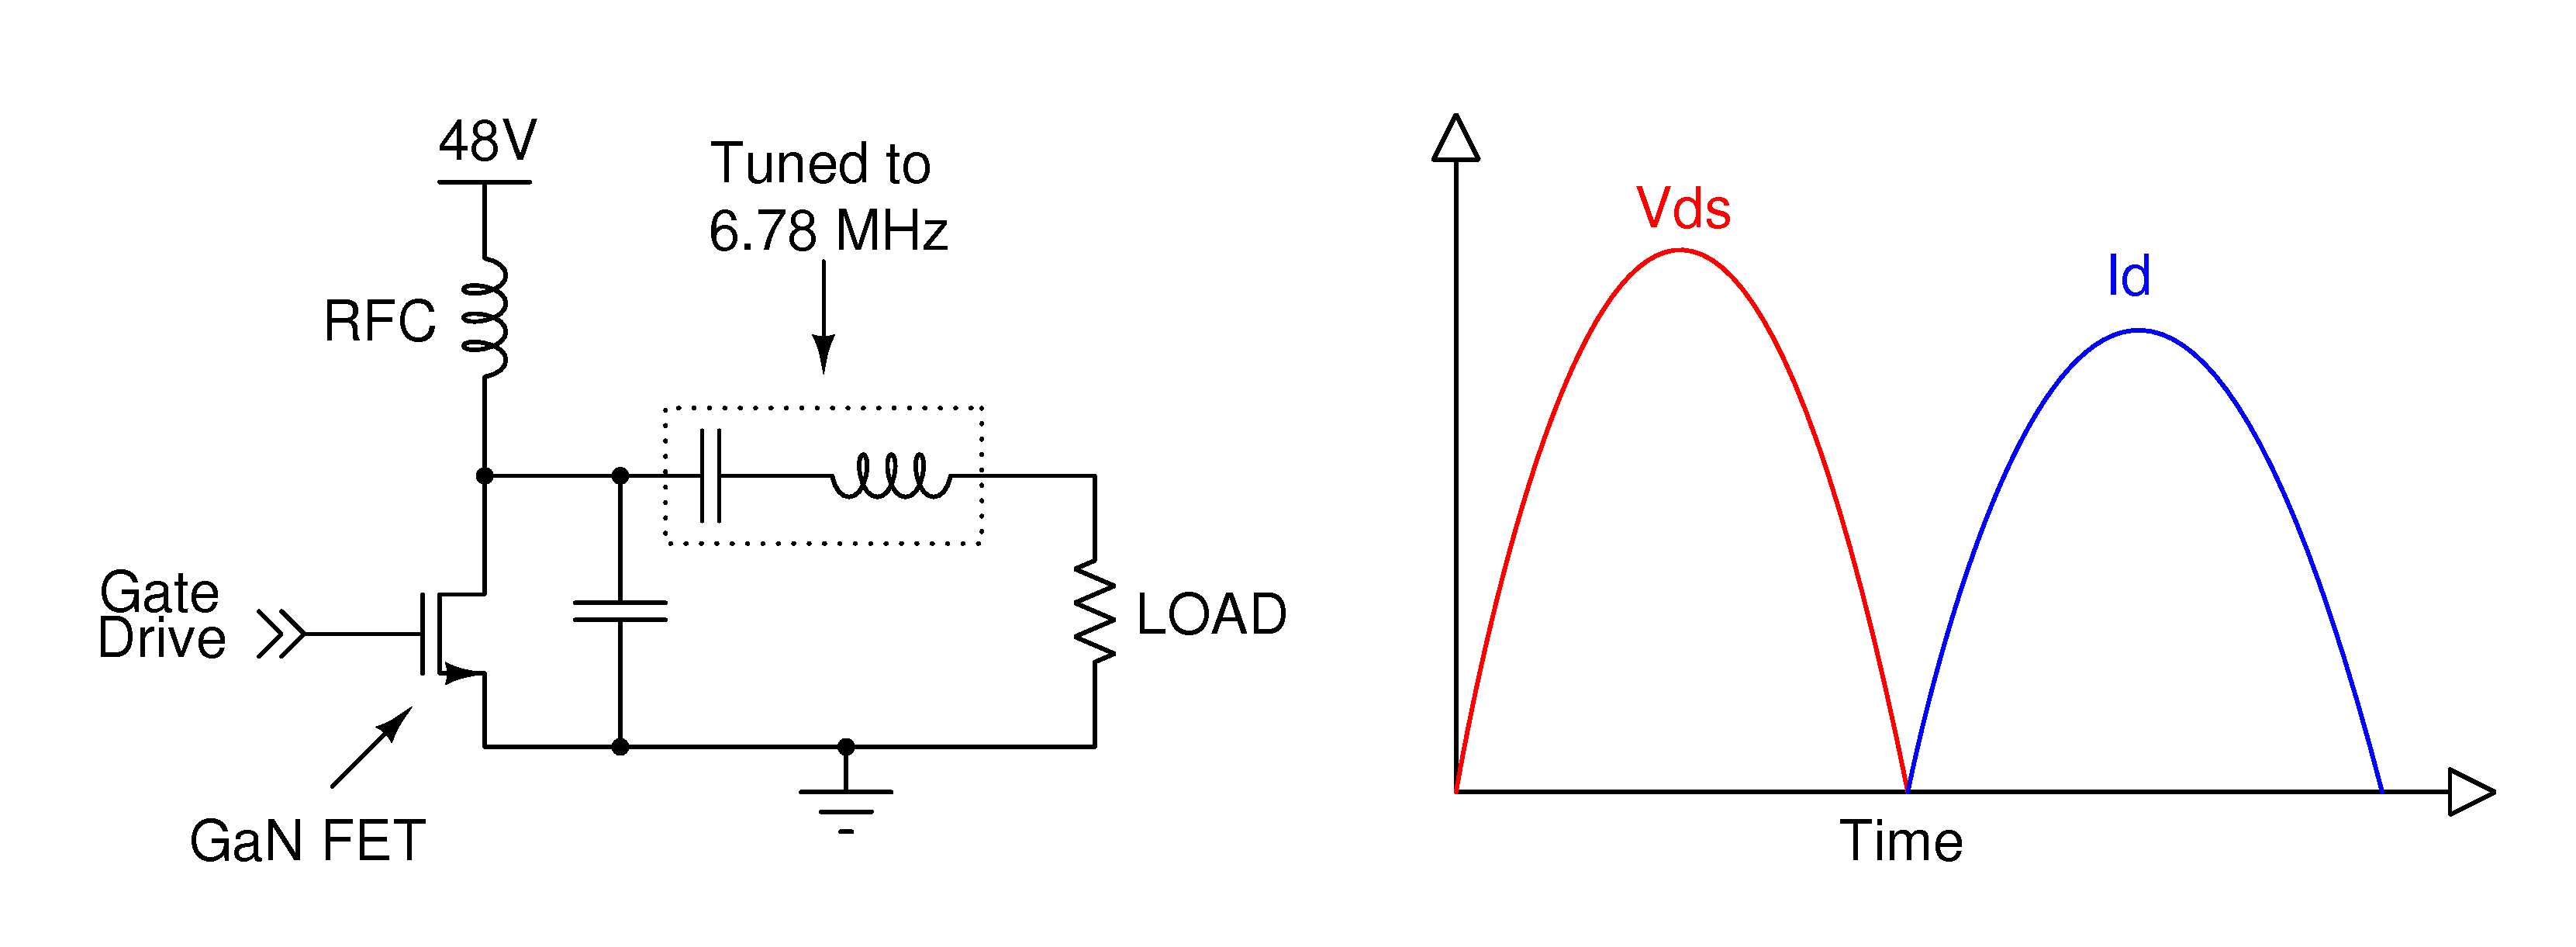
\includegraphics[scale=1.71644]{classE}\\
   % translate x=297 y=873 scale 0.22
   \putbox{1.93in}{2.09in}{1.20}{Amplifier Output}%
   \putbox{2.26in}{1.84in}{1.20}{Network}%
   \putbox{0.93in}{2.09in}{1.20}{RFC}%
   } % close 'parbox'
   } % close 'scalebox'
   \vspace{-\baselineskip} % this is not necessary, but looks better
